\documentclass[10pt,aspectratio=169]{beamer}

\usetheme{default}
\usecolortheme{seahorse}
\setbeamertemplate{navigation symbols}{}
\setbeamertemplate{footline}[frame number]
\setbeamerfont{frametitle}{size=\large,series=\bfseries}
\setbeamerfont{title}{size=\Large,series=\bfseries}

\usepackage{graphicx}
\usepackage{amsmath,amssymb}
\usepackage{booktabs}
\usepackage{xcolor}
\usepackage{tikz}

\definecolor{accent}{HTML}{C44E52}
\definecolor{good}{HTML}{4C7AB0}

\title{Beyond Representation:\\ Index Structure Limitations in Dense Retrieval}
\author{Alessandro Magnani}
\institute{AMLDS 2026 \;\textbar\; Osaka, Japan}
\date{July 2026}

\begin{document}

%% =====================================================================
\begin{frame}[plain]
  \titlepage
\end{frame}

%% =====================================================================
\begin{frame}{Why this talk}
  \begin{itemize}
    \item Dense retrieval is everywhere: e-commerce, enterprise search, RAG.
    \item Practical deployments rely on \textbf{approximate nearest-neighbor (ANN)} indices
          (HNSW, IVF) for speed.
    \item Most research focuses on the \emph{representation}---can the embedding
          capture the right semantics?
    \item This talk: \alert{the index itself imposes a separate, quantifiable failure mode}
          that disproportionately attacks a specific population of queries.
  \end{itemize}

  \vspace{0.5em}
  \begin{block}{Headline finding}
    Even when the embedding has enough representational capacity, switching from
    exact (Flat) to HNSW search forfeits \textbf{$\sim 63\%$ of achievable Recall@10}
    on identifier queries---vs.\ less than $2\%$ on standard queries.
  \end{block}
\end{frame}

%% =====================================================================
\begin{frame}{The two camps}
  \begin{columns}[T]
    \column{0.5\textwidth}
    \textbf{Sparse retrieval (BM25)}
    \begin{itemize}
      \item Inverted index over tokens.
      \item Exact lexical matching.
      \item Strong on rare terms, IDs, named entities.
    \end{itemize}

    \column{0.5\textwidth}
    \textbf{Dense retrieval}
    \begin{itemize}
      \item Continuous embedding + nearest-neighbor search.
      \item Strong semantic generalization.
      \item Indispensable in production for fluency \& multilinguality.
    \end{itemize}
  \end{columns}

  \vspace{1em}
  \begin{itemize}
    \item Prior theory (Tay et al.\ 2020; Fan et al.\ 2022):
          \emph{representation capacity} of dense models can match sparse---given
          enough dimensions.
    \item But: practical dense retrieval uses ANN, not exact search.\\
          \alert{What does that cost?}
  \end{itemize}
\end{frame}

%% =====================================================================
\begin{frame}{``Spear-fishing'' queries}
  \begin{block}{Definition (operational)}
    Queries whose relevance hinges on a single, low-frequency, high-IDF token:
    identifiers (SKUs, part numbers), rare terms, precise named entities.
  \end{block}

  \begin{itemize}
    \item In production: a small fraction of total traffic.
    \item But operationally critical: failures yield empty search-result pages,
          abandoned carts, broken RAG retrievals.
    \item In our experiments:
      \begin{itemize}
        \item \textbf{ID subset}: doc identifier used as query (extreme case).
        \item \textbf{Rare subset}: uni/bigram terms appearing in $\le 5$ docs.
        \item \textbf{Standard subset}: real user queries (control).
      \end{itemize}
  \end{itemize}
\end{frame}

%% =====================================================================
\begin{frame}{The mechanism: centroid dilution (theory)}
  IVF clusters the corpus into $N$ cells; at query time only the closest $n_{\text{probe}}$
  centroids are searched.

  \vspace{0.4em}
  Centroid of cluster $C$:\quad
  $c \;=\; \dfrac{1}{|C|}\sum_{d\in C} f(d) \;\;=\;\; \dots + \alpha_{t^*}\,p\,\phi(t^*) + \dots$

  \vspace{0.4em}
  For a query dominated by rare token $t^*$:
  \begin{equation*}
    \langle c, q\rangle \;\approx\; \alpha_{t^*}^2 \, p
      \;=\; \log^2\!\Big(\tfrac{M}{n_{t^*}}\Big)\cdot\frac{n_{t^*,C}}{M/N}
  \end{equation*}

  \vspace{0.3em}
  \begin{itemize}
    \item $\alpha_{t^*}$ is large for rare tokens (high IDF).
    \item But $p$ (in-cluster prevalence) is small for rare tokens.
    \item JL projection adds noise floor $\epsilon \approx \sqrt{\log V / d}$.
    \item \alert{Rare-token centroid signal lost when $\alpha_{t^*}^2 p \lesssim \epsilon$.}
  \end{itemize}

  \medskip
  \emph{Larger embedding $d$ helps $\epsilon$, but cannot fix small $p$.}
\end{frame}

%% =====================================================================
\begin{frame}{Experimental setup}
  \begin{columns}[T]
    \column{0.55\textwidth}
    \textbf{Datasets}
    \begin{itemize}
      \item \textbf{Home Depot}: 54{,}667 product titles
      \item \textbf{MS MARCO Passage v1.1}: 82{,}360 passages
    \end{itemize}

    \textbf{Three query subsets per dataset}\\
    (1{,}000 queries each)
    \begin{itemize}
      \item Standard \;\;\textbar\;\; Rare ($\le 5$ docs) \;\;\textbar\;\; ID
    \end{itemize}

    \column{0.45\textwidth}
    \textbf{Representation}
    \begin{itemize}
      \item Char-trigram + JL projection
      \item $d\in\{256, 512, 1024\}$
      \item Unsupervised
    \end{itemize}

    \textbf{Indices (FAISS)}
    \begin{itemize}
      \item Flat (exact)
      \item IVF (\texttt{nlist}, \texttt{nprobe} sweep)
      \item HNSW ($M{=}64$, \texttt{efC}/\texttt{efS})
      \item BM25 (Pyserini)
    \end{itemize}
  \end{columns}

  \vspace{1em}
  \begin{block}{Why unsupervised trigram, not DPR / Sentence-BERT?}
    A supervised encoder abstracts away the lexical detail that \emph{defines} a
    spear-fishing query. The Flat baseline would already fail on IDs---conflating
    representation failure with indexing failure. We need a representation that
    \emph{provably} preserves lexical distances (Johnson--Lindenstrauss).
  \end{block}
\end{frame}

%% =====================================================================
\begin{frame}{Headline result: the gap}
  \begin{center}
    \small
    \setlength{\tabcolsep}{6pt}
    \begin{tabular}{llrrrr}
      \toprule
      \textbf{Dataset} & \textbf{Subset} & \textbf{Flat} & \textbf{IVF} & \textbf{HNSW} & \textbf{BM25} \\
      \midrule
      HD       & standard & 0.327 & 0.314 & 0.321 & 0.447 \\
      HD       & rare     & 0.751 & 0.642 & 0.619 & 0.878 \\
      HD       & {\color{accent}\textbf{id}} & {\color{accent}\textbf{0.874}} & 0.590 & {\color{accent}\textbf{0.327}} & 1.000 \\
      \midrule
      MS MARCO & standard & 0.471 & 0.448 & 0.446 & 0.770 \\
      MS MARCO & rare     & 0.205 & 0.187 & 0.166 & 0.688 \\
      MS MARCO & {\color{accent}\textbf{id}} & {\color{accent}\textbf{0.174}} & 0.152 & {\color{accent}\textbf{0.071}} & --- \\
      \bottomrule
    \end{tabular}\\[4pt]
    {\footnotesize Recall@10 at $d{=}1024$, across-token trigrams, best ANN sweep config.}
  \end{center}

  \vspace{0.5em}
  \begin{itemize}
    \item Flat$\to$HNSW gap (relative):\;
          standard $\approx$ \textbf{2\%}\quad rare $\approx$ \textbf{18\%}\quad
          \alert{id $\approx 63\%$}.
    \item Same monotone pattern on both datasets.
    \item All gaps statistically significant (paired bootstrap $95\%$ CI excludes zero).
  \end{itemize}
\end{frame}

%% =====================================================================
\begin{frame}{Indirect evidence: IVF cluster granularity}
  \begin{columns}[T]
    \column{0.55\textwidth}
    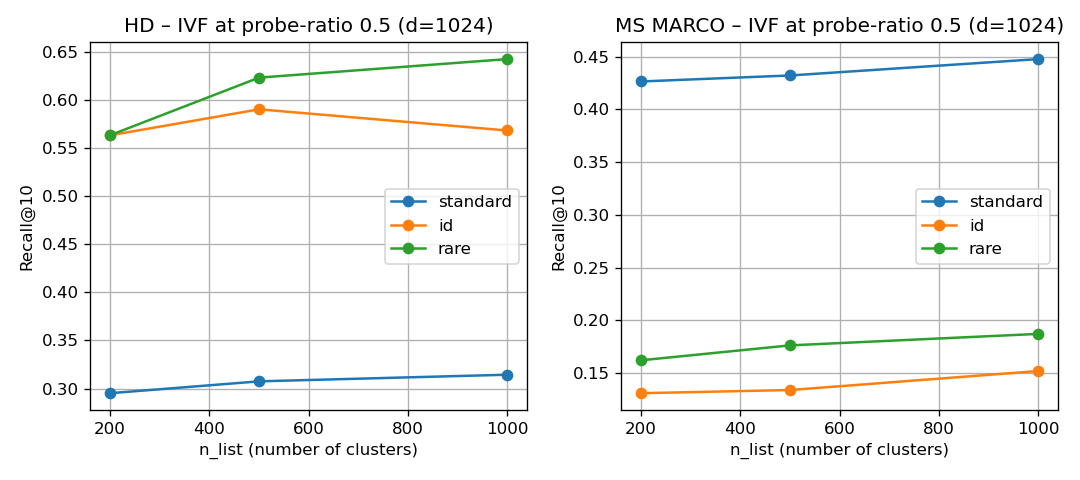
\includegraphics[width=\textwidth]{figures/ivf_nlist_sensitivity.png}

    \column{0.45\textwidth}
    \textbf{Theory predicts}: smaller clusters $\Rightarrow$ less centroid dilution
    $\Rightarrow$ rare/ID queries benefit more from finer clustering.

    \medskip
    \textbf{Data}: rare \& ID gain
    \emph{2--3$\times$ more} (relative) than standard going from
    $n_{\text{list}}{=}200 \to 1000$.

    \medskip
    Asymmetric improvement is exactly what Eq. (8) predicts.
  \end{columns}
\end{frame}

%% =====================================================================
\begin{frame}{Direct evidence: measure the centroid signal}
  \textbf{For each query}, compute the centroid signal
  $\langle q, c_{\text{rel}}\rangle$ on the centroid of the query's relevant
  cluster (IVF, $n_{\text{list}}{=}500$, $d{=}1024$).

  \begin{columns}[T]
    \column{0.55\textwidth}
    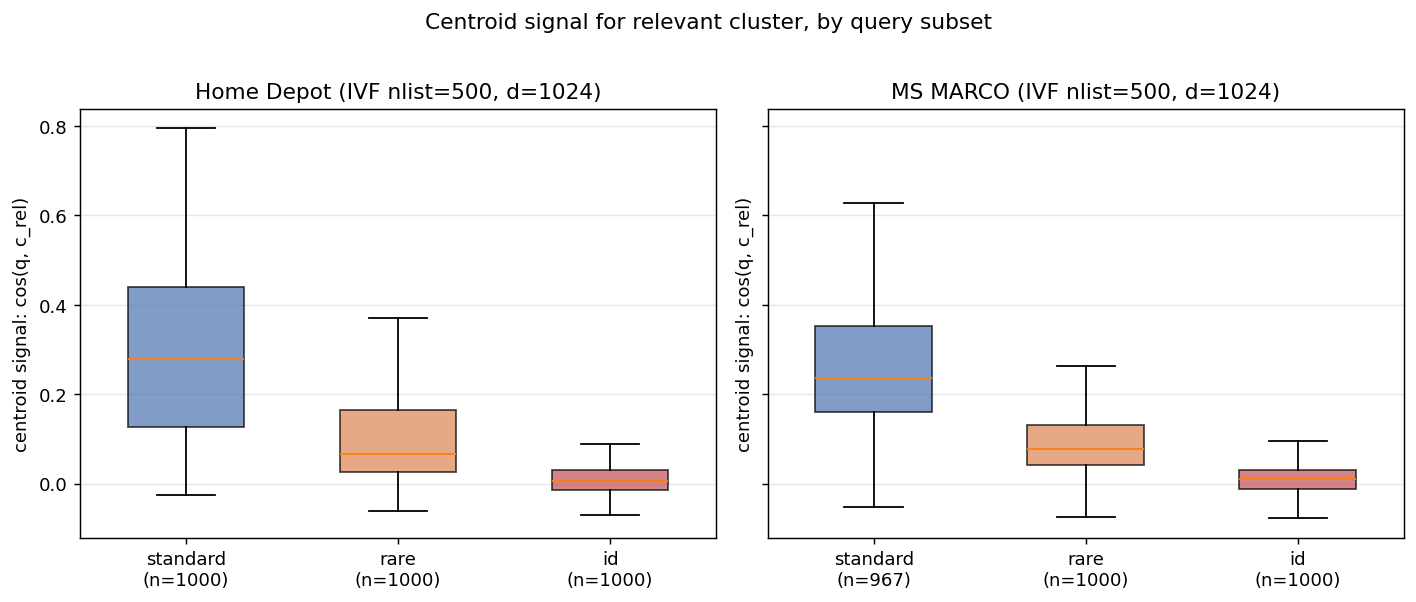
\includegraphics[width=\textwidth]{figures/centroid_signal_by_subset.png}

    \column{0.45\textwidth}
    \small
    \setlength{\tabcolsep}{3pt}
    \begin{tabular}{lrrr}
      \toprule
      Subset (HD) & signal & rank & hit@250 \\
      \midrule
      standard & 0.279 & 2   & 97\% \\
      rare     & 0.066 & 69  & 81\% \\
      \alert{id} & \alert{0.007} & \alert{216} & \alert{59\%} \\
      \bottomrule
    \end{tabular}

    \medskip
    \alert{$\sim 40\times$ collapse} from standard to ID:\\
    centroid signal disappears into the JL noise floor exactly as Eq.~(8) predicts.\\[0.3em]
    For HD-ID queries, $41\%$ of relevant clusters fall outside the top-half by centroid
    score---\emph{structurally unrecoverable}.
  \end{columns}
\end{frame}

%% =====================================================================
\begin{frame}{The empty-result rate}
  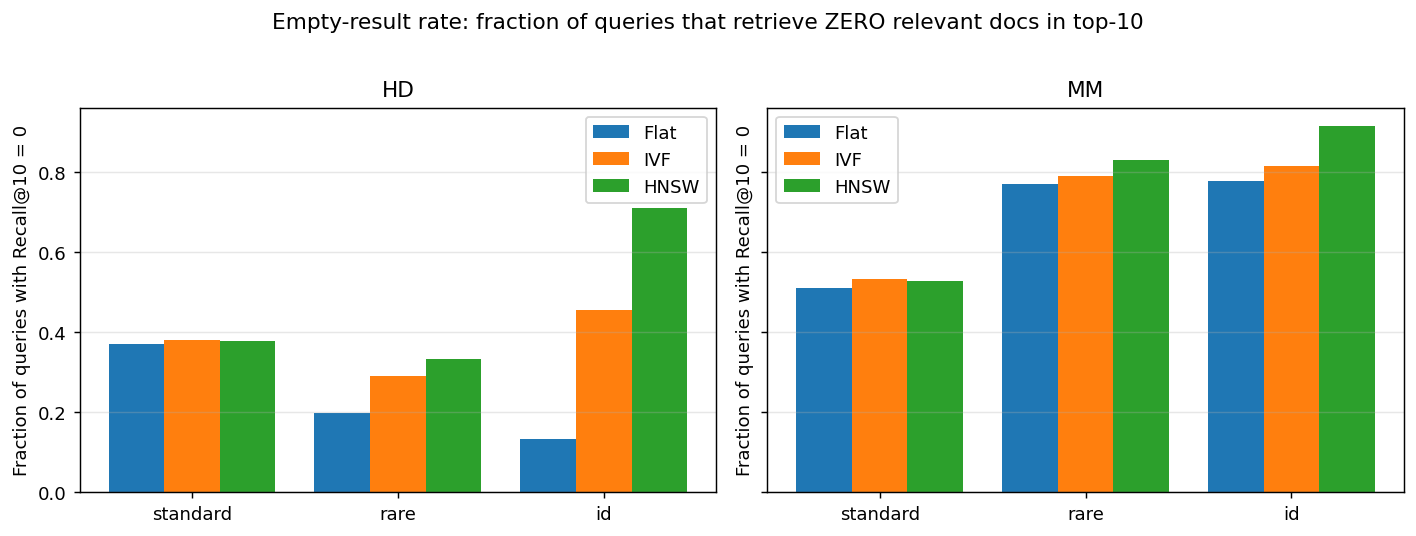
\includegraphics[width=\textwidth]{figures/D_zero_rate.png}

  \begin{itemize}
    \item HD-id Flat: \textbf{13\%} of queries return nothing relevant in top-10.
    \item HD-id \alert{HNSW: \textbf{71\%}}.
    \item Standard subset: barely moves.
    \item \emph{This is the production-visible symptom.}
  \end{itemize}
\end{frame}

%% =====================================================================
\begin{frame}{``But this is only because the embeddings are simple''}
  Reviewer question we anticipated: \emph{do learned dense encoders avoid this?}

  \medskip
  Re-ran the full grid with \texttt{all-MiniLM-L6-v2} (Sentence-BERT, 384-dim, supervised).

  \medskip
  \begin{center}
    \small
    \setlength{\tabcolsep}{6pt}
    \begin{tabular}{llrr}
      \toprule
      Dataset & Subset & Trigram Flat R@10 & \textbf{MiniLM Flat R@10} \\
      \midrule
      HD       & standard & 0.327 & 0.298 \\
      HD       & rare     & 0.751 & 0.428 \\
      HD       & {\color{accent}id} & {\color{good}0.874} & {\color{accent}\textbf{0.010}} \\
      MS MARCO & standard & 0.471 & {\color{good}\textbf{0.894}} \\
      MS MARCO & rare     & 0.205 & 0.226 \\
      MS MARCO & {\color{accent}id} & {\color{good}0.174} & {\color{accent}\textbf{0.001}} \\
      \bottomrule
    \end{tabular}
  \end{center}

  \vspace{0.5em}
  \begin{itemize}
    \item MiniLM nearly doubles MS MARCO standard recall---as designed.
    \item MiniLM \textbf{cannot distinguish identifiers}: ``12345'' $\approx$ ``67890''.
    \item Representation collapses \emph{before} the index has a chance to bias.
    \item This is exactly why a supervised encoder is the \emph{wrong instrument}
          for our study---and exactly why hybrid retrieval is needed in production.
  \end{itemize}
\end{frame}

%% =====================================================================
\begin{frame}{What this means for production}
  \begin{block}{Translation: lost user sessions}
    Switch from exact to HNSW at fixed embedding quality, you forfeit:
    \begin{itemize}
      \item $\sim 63\%$ of achievable recall on identifier queries,
      \item $\sim 18\%$ on rare-term queries,
      \item $\sim 2\%$ on standard queries.
    \end{itemize}
    Average-case recall reported with an ANN deployment substantially
    \emph{overstates} worst-case service quality.
  \end{block}

  \medskip
  \textbf{Recommendations:}
  \begin{enumerate}
    \item \emph{Query-type-aware routing}: send spear-fishing traffic to BM25 / Flat.
    \item \emph{Index-aware training}: penalize placement of rare features in
          poorly-reachable embedding regions.
    \item \emph{Hybrid retrieval}: sparse for precision on rare tokens, dense for
          semantic generalization. Not new advice---but now with a quantitative justification.
  \end{enumerate}
\end{frame}

%% =====================================================================
\begin{frame}{Takeaways}
  \begin{enumerate}
    \item Representation capacity is \emph{necessary but not sufficient} for
          production dense retrieval.
    \item ANN indices introduce a \emph{second}, structurally different failure mode
          that concentrates on rare-token / identifier queries.
    \item We formalized this as \textbf{indexing bias} and derived a
          \textbf{centroid-dilution bound} that we then directly measured per query.
    \item The Flat$\to$HNSW gap on identifier queries is $\sim 30\times$ larger
          than on standard queries, in both retail and open-domain text.
    \item Supervised encoders don't escape this---they collapse at the
          representation stage on the same queries.
  \end{enumerate}

  \vfill
  \begin{center}
    \large
    \textbf{Code \& experiments:} \texttt{github.com/alemagnani/sparse-dense-paper}
  \end{center}
\end{frame}

%% =====================================================================
\begin{frame}[plain]
  \begin{center}
    \vspace{2em}
    {\Huge \bfseries Thank you}\\[1em]
    {\large Questions?}\\[2em]

    \small Alessandro Magnani \;\textbar\; \texttt{ale.magnani@gmail.com}\\
    AMLDS 2026 \;\textbar\; Osaka, July 2026
  \end{center}
\end{frame}

\end{document}
